\chapter{Projekt}
\section{Architektura}
Architektura rozwiązania. Aplikacja stworzona będzie w architekturze klient-serwer. Interfejs użytkownika zrealizowany będzie w technolgii aplikacji internetowych, tak by dostęp do repozytorium nie wymagał instalacji i był dostępny na wszystie platformy. Dodatkowo stworzona zostanie usługa internetowa ( ang. web service ), tak by umożliwić zintegorowanie aplikacji z zewnętrznymi aplikacjami dzięki czemu możliwa będzie automatyzacja kluczowych procesów. Perzystencja danych dokonywana będzie w relacyjnej bazie danych poprzez moduł odwzorowujący obiektową architekturę systemu informatycznego na bazę danych.

Aplikacja zostanie napisana w języku JAVA. Język ten jest obecnie najczęśniej spotykanym językiem w zagadnieniach korporacyjnych. Posiada rozwinięte wsparcie społeczności i rozbudowane funkcjonalności wbudowane, jak i rozwijane przez zewnętrznych kontrybutorów. 
\begin{figure}[h]
\centerline{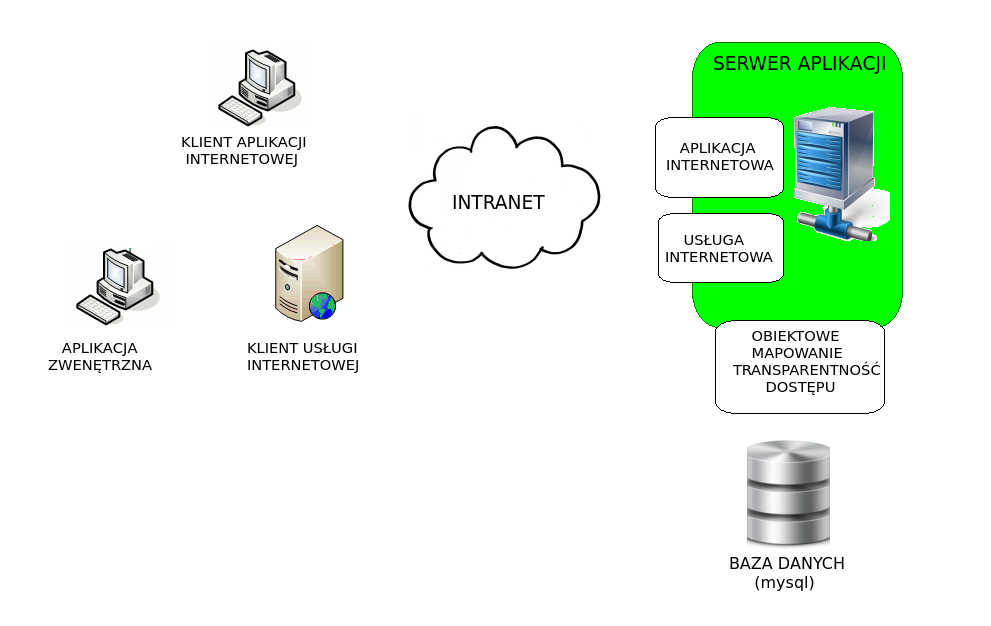
\includegraphics[scale=0.5]{img/architektura.png}}
\caption{Architektura systemu}
\label{fig:architektura}
\end{figure}


%<< Diagram fizyczny >>

%<< Diagram komponentów >>

%Komponent zarządzanie użytkownikami

%Komponent Definicji 

%Komponent wykonania testów

%Komponent danych dodatkwych
\section{Warstwy}
\subsection{Warstwa aplikacji internetowej}
Dostęp poprzez aplikację internetową jest podstawowym źródłem interakcji użytkowika w projektowanej aplikacji. Celem rozdzielenia poszczególnych odpowiedzialności modułów oprogramowania, użyty zostanie zworzec Model-Widok-Kontroler. Zakłada on wydzielenie trzech wartst:
\begin{enumerate}
  \item Model - odpowiedzialny za pobranie i enkapsulacje danych
  \item Widok - odpowiedzialny za wyświetlenie sformatowanej treści. Język stosowany w widoku powinien pozwalać na swobodne osadzanie treści języka końcowego ( w tym przypadku HTML ), powinien on być dostosowany do edycji przez osoby nie posiadające wiedzy na temat języku programowania.
  \item Kontroller - odpowiedzialny za skoordynowanie pobrania danych, przetworzenia ich za pomocą serwisów i przesłanie danych do widoku
\end{enumerate}

Język JAVA oferuje kilka ustandaryzowanych technologii które pozwalają tworzyć aplikacje internetowe z wykorzystaniem wzorca Model-Widok-Kontroler. Zaprezentowana aplikacja stworzona zostanie w oparciu o technologię Java Server Faces i jej implementacje PrimeFaces.

Java Server Faces jest jednym ze standardów tworzenia aplikacji internetowych w języku JAVA\cite{jsfRef}. Główne założenia standardu to:
\begin{enumerate}
  \item Łatwość tworzenia części klienckiej ( widoku ) w oparciu o strukturę komponentową. Udostępnione są standardowe komponenty ( takie jak na przykład formularz, pole tekstowe ).
  \item Możliwość zagnieżdżania struktury dokumentu, pozwalająca na minimalizację redundancji po stronie szablonu strony internetowej 
  \item Ustandaryzowany dostęp z widoku do danych po stronie serweru
  \item Zapewnienie trwałości stanu danych pomiędzy żądaniami w obrębie sesji klienta
  \item Część serwerowa oparta jest na ziarnach ( JavaBeans ), posiada wsparcie dla walidacji zarówno po stronie klienckiej jak i serwerowej
\end{enumerate}

W technologii Java Server Faces rola Kontrolera rozdzielona jest na pliki szablonu strony i ziarna zarządzające po stronie serweru. W plikach szablonu osadzone są instrukcję które wprost pobierają danę z kontrolera i wykonują na nim akcje.

Standard Java Server Faces posiada wiele implementacji. W tworzonej aplikacji użyta została implementacja PrimeFaces\cite{primeFaces}. PrimeFaces jest rozwijany jako otwarty projekt. Implementacja ta rozszerza standard o własne komponenty, uproszcza również sposób komunikacji klient serwer poprzez AJAX ( asynchroniczna komunikacja poprzez język JavaScript)

\subsection{Warstwa usługi internetowej}



Jedym ze standardów komunikacji między aplikacjami jest komunikacja poprzez usługę internetową, dla której istnieje wiele technologii. W niniejszej pracy użyta zostanie technologia REST. REST zakłada iż deklaracja działania które klient zamierza osiągnąć po stronie serwera określona jest w dwóch miejscach:
\begin{enumerate}
  \item URI czyli adres interntetowy określa do którego zasobu odwołuje się klient
  \item  typ metody HTTP ( zgodnie z HTTP/1.1) określa jakie działanie ma być podjęte na zasobie ( wyświetlenie, dodanie, modyfikacja, usunięcie)
\end{enumerate}

Zgodnie ze specyfikacją HTTP/1.1 możemy wyróżnić następujące metody i oczekiwany rezultat po stronie serwerowej:

\renewcommand\multirowsetup{\centering\arraybackslash}
\begin{longtable}{|c|c|}
\hline
\textbf{metoda} & \textbf{mapowanie na akcje} \\ \hline
GET & Wyświetlenie, pobranie zasobu \\ \hline
PUT & Stworzenie zasobu \\ \hline
POST & Modyikacja zasobu \\ \hline
DELETE & Usunięcie zasobu \\ \hline
OPTIONS, TRACE, HEAD & nie używane \\ \hline

\caption{Metody HTTP/1.1 \cite{http}}
\end{longtable}

Poprzez usługę internetową możliwe będzie wykonanie następujących akcji:
\begin{enumerate}
  \item dodanie wymagania
  \item pobrania listy przypadków testowych do wykonania dla użytkownika
  \item aktualizacji wykonania przypadku testowego
\end{enumerate}
Pierwszy punkt pozwala na integracje z aplikacją przechowującą wymagania. Punkt drugi i trzeci pozwala na integracje z zewnętrznymi aplikacjami do wykonywania testów. W szczególnym przypadku poprzez stworzenie fikcyjnego użytkownika np. automatyzacja, można zintegrować repozytorium z modułem wykonującym testy automatycznie.


\section{Moduły aplikacji}
Funkcjonalności realizowane przez aplikację możemy podzielić na logicznę moduły.
\begin{figure}[h]
\centerline{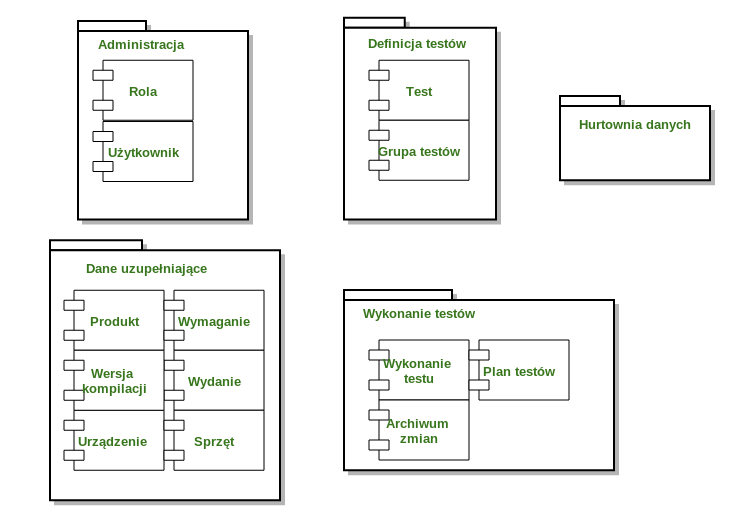
\includegraphics[scale=0.5]{img/komponenty.png}}
\caption{Mouły systemu}
\label{fig:moduly}
\end{figure}

\subsection{Moduł administracji}

Moduł ten skupia wszelkie funkcjonalności związane z zarządzaniem użytkownikami w systemie. Odpowida za tworzenie i edycję użytkowników. Każdy użytkownik posiada takie dane jak login, adres e-mailowy, hasło jak również przypisaną rolę.

Możemy wyróżnić kilka ról użytkowników. Rola określa jakie uprawnienia otrzymuje zalogowany użytkownik i określa widok ekranu początkowego. Każda z ról posiada charakterystyczne cechy które pokrywają role użytkowników w procesie testowania oprogramowania: menedżer testów, lider testów, inżynier testów, specjalista środowiska do testów, specjalista konfiguracji testowej \cite{peopleWare}. Poniżej zaprezentowany zostanie opis poszczególnych ról.
\begin{enumerate}
  \item Administrator --  zarządza użytkowikami w systemie. Administrator tworzy użytkowników i nadaje im uprawnienia.
  \item Koordynator testów -- tworzy przypadki testowe, grupy testów i plany testów. Rola ta odpowiedzialna jest za treści merytoryczne repozytorium. Użytkownik odpowiada za utrzymanie testów, aktualizację ich, pokrycie funkcjonalności. 
  \item Obsługa techniczna -- rola ta odpowiedzialna jest za zapewnienie odpowiedniego środowiska dla testerów, konserwacje i naprawę fizycznych defektów. Użytkownik ten przypisany jest do konkretnych wykonań scenariuszy, instaluje początkowe środowisko, wymagane wersje oprogramowania, naprawia usterki sprzętowe.
  \item Lider testów -- wspiera zespół w wykonynwaniu planu testów testowego. Służy swoją wiedzą i doświadczeniem przy podziale prac i podczas pojawiających się problemów. Posiada władzę decyzyjną przy zakwalifikowaniu testu jako nie udanego. Lider przypisuje testerów do testów.
  \item Tester --  wykonuje przypisane do niego przypadki testowe. Odznacza stan testów i zgłasza napotkane problemy.
  \item Pośrednik ( ang. liaison ) --  Odpowiedzialny jest za komunikacje zespołu testów z zespołem programistycznym. Posiaga wgląd do aktulnie wykonywanyh testów i konfiguracji. Jego zadaniem jest rozwiązywanie problemów związanych z jego macierzystym produktem. Pomaga zakwalifikować problem powstały podczas testów, szczególnie na początku testów produktu, zespół testerki może nie posiadać wystarczającej wiedzy i błędnie kwalifikować obserwowane rezultaty jako błąd produktu. Pośrednik proponuje również tymczasowe rozwiązania które pozwalają obejść problemy wynikające z błędów w oprogramowaniu, które naprawione będą dopiero podczas przyszłych wersji oprogramowania, tak by proces testowania mógł przebiegać nieprzerwanie.
\end{enumerate}
  
\subsection{Moduł definicji}

Moduł ten jest odpowiedzialny za definicję podstawowych jednostek systemu czyli: testów, grup testów i planów testów. 

Podstawową jednostą aplikacji jest przypadek testowy. 
\begin{longtable}{| p{6cm}  | p{10cm} |}
 \hline 
\textbf{Nazwa elementu} & \textbf{Opis}  \\ \hline
\endfirsthead
\multicolumn{2}{c}%
{\tablename\ \thetable\ -- \textit{Kontynuacja}} \\
\hline
\\textbf{Nazwa elementu} & \textbf{Opis}  \\
\hline
\endhead
\hline \multicolumn{2}{r}{\textit{Kontynuacja na następnej stronie}} \\
\endfoot
\hline
\endlastfoot
  identyfikator & jednoznacznie identyfikujący test, unikatowy ciąg znaków \\ \hline
  tytuł & tytuł testu \\ \hline
  abstrakt & czyli opis testu, jego kluczowe założenia, tematyka i tło określające test \\ \hline
  grupy urządzeń & Do jednej grupy urządzeń może być przypisane jedno lub więcej urządzeń ( w przypadku gdy dana funkcjonalność adresowana jest na więcej niż jedno urządzenie danego typu). Podczas wykonania testu należy jednak określić którego urządzenia z grupy należy użyć ( wybrać jedno)\\ \hline
  stan wejściowy konfiguracji & Definiowane jest tutaj sprzęt i jego stan który jest wymagana do wykonania testu. Dla każdego ze stanów można zdefiniować warunek określający dla jakich konfiguracji grup urządzeń stan ma zajść \\ \hline
   scenariusz &  lista kroków do wykonania wraz z oczekiwanymi rezultatami \\ \hline
    wymagania & lista wymagań które są weryfikowane poprzez wykonanie testu \\ \hline
    estymowany czas & estymowany czas potrzebny do wykonania przypadku testowego \\ \hline
     stan początowy produktów & stan początkowy poszczególnych produktów który musi być spełniony. Dla każdego ze zdefiniowanych stanów możliwe jest przypisanie warunku który określa dla jakiej konfiguracji grup urządzeń stan ma zajść \\ \hline
     ilość wariacji & ilość możliwych alternatywnych przebiegów przypadku testowego ( w zależności od doboru urządzeń ) \\ \hline \hline
 \caption{ Składowe przypadku testowego}
\end{longtable}


Przypadki testowe wchodzą w skład grup testów. Hierarchia ta ma drzewiastą strukturę co oznacza iż grupy mogą być zagnieżdżane. Grupy powinny agregować testy które posiadają podobną charakterystykę. Na przykład testują te same funkcjonalności, wymagają podobnej konfiguracji, urządzeń, dokumentacji. Testy funkcjonalne i niefunkcjonalne nie powinny znajdować się w tym samym przypadku testowym. Składowe:

\begin{longtable}{| p{6cm}  | p{10cm} |}
 \hline \hline
\textbf{Nazwa elementu} & \textbf{Opis}  \\ \hline
  identyfikator & jednoznacznie identyfikujący grupę, unikatowy ciąg znaków \\ \hline
  identyfikator rodzica & grupy mogą przybierać postać drzewiastą \\ \hline
  tytuł & tytuł grupy testowej \\ \hline
  opis & opis grupy testowej, określający jakiego typu testy powinny znaleźć się w grupie \\ \hline
 \caption{ Składowe grupy testów}
\end{longtable}


\subsection{Moduł danych uzupełniających}

Definicja testów przez swoją złożoność i potrzebę pełnej specyfikacji wymaga pewnych danych dodatkowych które muszą zostać zdefiniowane w aplikacji. Repozytorium przeznaczone jest dla systemów wielo wydaniowych i wspierany jest inkrementacyjny model wytwarzania oprogramowia.

Pierwszym krokiem jest zdefiniowanie produktów wchodzących w skład systemu który poddany zostanie testom. System w kontekście aplikacji jest to zbiór zintegrowanych produktów które współdziałając oferują określoną funkcjonalność z perspektywy klienta.

W celu wsparcia inkremetacyjnego modelu wytwarzania oprogramowania w aplikacji istnieją takie elementy jak "wydanie produktu" i "wersja produktu" która wchodzi w skład wydania. Poprzez wersje produktu rozumiany jest konkretny skompilowany stan kompontów systemu. Wersja systemu powina być jednoznacznie identyfikowalna ponieważ stanowi linie bazową. Na podstawie porównania dwóch poprzedzających się wersji można określić kiedy został wprowadzony błąd regresji. Wydania produktu są to wersje widocznę z poziomu klienta końcowego, w ich skład najczęśniej wchodzi wiele wersji.

W ramach wydań produktów definiowane są wymagania. Wymaganie powinno być jasno zdefiniowane tak by możliwe było zweryfikowanie spełnienia wymagania przez oprogramowanie. Na podstawie wymagań tworzone są przypadki testowe.

Drugą charakterystyką aplikacji jest wsparcie dla systemów dedykowanych na wiele urządzeń. Aplikacje umożliwia więc przechowywanie informacji o urządzeniach. Definicja urządzenia powinna zawierać dane podstawowe takie jak nazwa, dostawca, zdjęcie jak i referencję do kompletnej dokumentacji na temat urządzenia. Dostęp do dokumentacji jest kluczowy podczas testów, szczególnie dla młodego stażem zespołu testerskiego.

W module definicji testów, podczas tworzenie przypadku testowego tworzone są grupy urządzeń. W skład grupy może wejść jedno lub więcej urządzeń, przy czym podczas wykonania przypadku testowego należy wybrać tylko jedno urządzenie dla każdej z grup. Konfiguracja wybranych urządzeń determinuje i modyfikuje końcową treść przypadku testowego. Od tego które urządzenia zostały wybrane mogą zależeć poszczególne kroki, stany początkowe produktów i wymagany sprzęt. Aplikacja repozytorium udostępnia sposób definiowania warunków dla wcześniej wspomnianych elementów. Warunek określa iż dany element jest ważny ( wchodzi w skład definicji przypadku testowego) wtedy i tylko wtedy gdy dla określonej grupy urządzeń wybrane zostało określone urządzenie.

Jednym z elementów wykonania testów funkcjonalnych jest instalacja środowiska do wykonania testów. Instalacja składa się z kilku elementów:
\begin{itemize}
  \item dostarczenie i zainstalowanie sprzętu wymaganego do wykonania testów ( przykładowo może to być symulator fal radiowych, sejf automatyczny, kabel ethernet, komuter stacjonarny )
  \item instalacja platformy do wykonania testów ( systemy operacyjne, środowiska uruchomieniowe, modyfikacji systemów, bios, maszyny wirtualne )
  \item instalacja oprogramowania w wersji zgodnej z planem testów
\end{itemize}

\subsection{Moduł wykonania }

Moduł ten przechowuje informacje o realizowanych planach testowych, testach oczekujących do wykonania i historie wykonywanych przypadków testowych.

Pierwszym krokiem jest utworzenie planu testów. Plan testów określa ramy testów, definiuje co i dlaczego powinno zostać przetestowane, określa konfigurację środowiska testowego.

\begin{longtable}{| p{6cm}  | p{10cm} |}
 \hline \hline
\textbf{Nazwa elementu} & \textbf{Opis}  \\ \hline
  identyfikator & jednoznacznie identyfikujący plan, unikatowy ciąg znaków \\ \hline
  tytuł & tytuł plan \\ \hline
  opis & opis planu testowego \\ \hline
  wymagania & lista wymagań których spełnienie zostanie zweryfikowane podczas przeprowadzania testów \\ \hline
  urządzenia & lista urządzeń dostępnych podczas testów \\ \hline
  wersja systemu & wersja systemu która będzie wdrożona podczas testowania  \\ \hline
 \caption{ Składowe planu testów}
\end{longtable}



Po utworzeniu planu testowego należy przypisać do planu testy które mają zostać wykonane. Wybóru należy dokonać biorąc po uwagę potrzebę spełnienia planu przy określonych zasobach ludzkich, pokrycia wymagań i ograniczeń wynikających z dostępności sprzętu i urządzeń.

Plan testów określa jakie wymagania należy zweryfikować, jest to kluczowy aspekt podczas doboru przypadków testowych. Należy dobrać takie przypadki testowe które weryfikuję potrzebne wymagania. Na tym jednak dobór przypadków testowych nie powinien być zakończony. Należy pamiętać o potrzebie przeprowadzenia regresji. Fakt iż określona wersja systemu dostarcza pewne funkcjonalności nie oznacza iż poprzednio przetestowane funkjonalności dalej działają poprawnie.

Podczas przypisania przypadku testowego do planu, należy go dookreślić w przypadku gdy posiada grupy urządzeń złożone z więcej niż jednego urządzenia. Oznacza to iż należy wybrać jedno i tylko jedno urządzenie dla każdej z grup. Wybór z jednej strony warunkowany jest dostępnymi zasobami sprzętowymi, a z drugiej strony powinien uwzględniać przetestowanie wszerz systemu dla różnych konfiguracji sprzętowych. Nalaży unikać w sytuacji w której nie zostaną wykonane testy na urządzeniach które są poprawne z perspektywy klienta.

Po dokonaniu pełnej definicji przypadku testowego, rozwiązywane są wszystkie warunki określone w takich elementach jak: stany produktu, kroki testu, warunki początkowe. Dla przypomnienia dla tych elementów można określić warunki które stanowią iż dany element wchodzi w skład przypadku testowego wtedy i tylko wtedy gdy dostępna jest konkretna konfiguracja sprzętowa ( wybrane zostało konkretne urządzenie z grupy urządzeń ). Schemat dla stanów produków można przedstawić na zamieszczonym poniżej pseudokodzie.

	\begin{codebox}
	\li \For{$stanProduktu$ \kw{in} $stanyProduktu$}
	\li \Do   
	\For{$warunek$ \kw{in} $warunkiDlaGrupUrzadzen$}
	\li \Do
	     \If $wybraneUrzadzenie  ==  preferowaneUrzadzenieDlaStanu$
	\li     \Then
	           $\proc{dodaj-stan-do-testu}(stanProduktu)$	         	         
	        \End	        
	\li  \End	 
	\li
	  \End
	  
	\end{codebox}
%	\caption{ Alogrytm doboru stanów produkto do przypadku testowego }

Rezultat wykonania przypadku testowego może przyjmować jedną wartość z podanych:
\begin{itemize}
   \item oczekujący - przypadek testowy oczekuje na przypisanie przez testera ( każda osoba z zespołu może się przypisać )
   \item przypisany - przypadek testowy przypisany do testera ( przypadek nie jest już widoczny w puli )
   \item zablokowany - przypadek testowy zablokowany przez błąd w innym przypadku, bądź poprzez niegotową konfigurację
   \item rezultat pozytywny - wszystkie kroki scenariusza wygenerowały oczekiwane rezultaty
   \item rezultat negatywny - przynajmniej jeden z kroków scenariusza wygenerował rezultat negatywny, lub testy eksporacyjne związane z przypadkiem testowym wygenerowały rezultat negatywny
   \item nie możliwy do wykonania - przypadek niemożliwy do wykonania z przyczyny braku zasobów
   \item wymagana analiza - podczas wykonywania przypadku testowego, wyniki poszczególnych kroków scenariusza nie dały jednoznacznej odpowiedzi. Wymagana jest konsultacja lidera i pośrednika ( ang. liaisona)
 \end{itemize} 

Po wykonaniu przypadku testowego, tester oznacza wynik wykonania przypadku testowego i w razie konieczności opisuje wnioski jako komentarz. Tester uzupełnia też realny czas poświęcony na wykonanie przypadku testowego.

\subsection{ Moduł hurtowni danych  }

Moduł ten odpowiedzialny jest za interpretacje danych istniejących w repozytorium. Przedstawiane są tutaj metryki i wykresy kluczowe z perspektywy lidera, koordynatora i kierownika testów.

Pierwszą z grup raportów jest wykres pokrycia wymagań na poziome deinicji testów. Analiza pozwala określić które części wymagań nie są pokryte przez przypadki testowe.

Drugą grupą jest pokrycie wymagań na podstawie wykonania przypadków testowych. Pokrycia można analizować odpowiednio z poziomu pojedyńczego planu testów, grupy testów i całego wydania systemu. Dane te dostarczają informacji na temat tego które z wymaganych obszarów zostały pokryte podczas rzeczywistych testów. Dzięki tym informacją kierownik zespołu testów może zaplanować zakres kolejnych planów testów.

Trzecia grupa dotyczy relacji pomiędzy urządzeniami a przypadkami testowymi. Analiza danych dostarczanych w tej grupie pozwala określić które urządzenia zostały już przetestowana a także które urządzenia należy dostarczyć i włączyć w przyszłych przypadkach testowych.

Czwarta grupa dotyczy procentowego stanu przypadków testowych. Analiza danych dostarczanych przez tą grupę pozwala określić czy wraz z czasem projektu zmniejsza się liczba znajdywanych defektów, określić procent testów zablokowanych i inne wnioski które mogą wpłynąć na zwiększenie efektywności zespołu testerskiego.



\chapter{Implementacja}
// TODO
Interfejs użytkownika stworzony został w technologi aplikacji internetowych przy użyciu technologii Java Server Faces która realizuje wzorzec projektowy  Model-Widok-Kontroler. Warstwa serwerowa działa na serwerze aplikacji Glassfish. Silnik bazodanowy to Mysql, silnik ten może być zmieniony podczas wdrożenia aplikacji poprzez zastosowanie tranparentności dostępu do danych. Moduł odwzorowujący obiektową architekturę systemu informatycznego na bazę danych udostępnia wiele implementacji baz danych przy czym interfejs jest wspólny.

\chapter{Przypadki użycia aplikacji}
// TODO 
\begin{enumerate}
  \item Tworzony jest nowy projekt
  \item Tworzone są wymagania
  \item Na podstawie wymagań tworzone są grupy testów i przypadki testowe. Scenariusze przypadków testowych tworzone są przy współpracy z zespołem programistycznym.
  \item Tworzony jest nowy plan testów który testować będzie nowe wydanie produktu. Tworzony jest harmonogram uwzlględniający poszczególne inkrementy produktu i testowane funkcjonalności.
  \item Do planu testów dodawane są testy. Podczas dodawania testów należy wziąć pod uwagę pokrycie nowych funkcjonalności i równomierne rozplanowanie testów dla różnych urządzeń.

\end{enumerate}

\chapter{Wnioski i możliwości rozwoju aplikacji}
